\documentclass{article}
\usepackage{graphicx,wrapfig,lipsum}

\usepackage[colorlinks = true,
            linkcolor = blue,
            urlcolor  = blue,
            citecolor = blue,
            anchorcolor = blue]{hyperref}

\begin{document}

\title{\textbf{Journal 1}}
\author{Ahmed Al Guqhaiman}
\date{\today}
\maketitle

\begin{wrapfigure}{r}{1.5in}
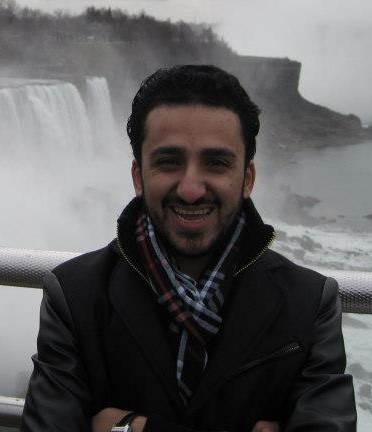
\includegraphics[width=1.5in]{Niagara_Falls.jpg}
\end{wrapfigure} 
{\lipsum[0-0]

The computer science research class is the first research course I have ever taken. Thus, it will be very helpful for me as a graduate student throughout my research journey. I hope to learn the most effective research methods for the most common computer science dissertations Learning the differences between qualitative, quantitative, and mixed methods in details with the most effective tools in each approach are also critical. How to find and select the most suitable workshops, conferences, and journals is extremely important. I also would like to distinguish the good venues from the bad ones. Moreover, I need to learn how to read and write papers more effectively. In particular, I need to learn how to develop a thesis proposal, develop a hypothesis, define a good problem statement, collect and analyze data, find the appropriate data set, use the results to make a qualitative or quantitative conclusion, do statistical analysis, and present research paper more effectively. Investigating a problem can be done through questionnaires and interviews. In either approach, when the number of participants will be enough to generalize the results and be publishable in a good venue. In this type of research, I would also like to learn how to deal with the incomplete survey, combine data from multiple sources, analyze the survey data, collect data more effectively. At the end of this semester, I hope that my research paper meets the standard to get accepted for publication in a top rank conference. I am a Ph.D. student in the Engineering Security program. This year is my junior year and my research interests lie in the Media Access Control (MAC) protocols, routing protocols, Software Defined Network (SDN), and network security. I just became a father to a beautiful baby girl four months ago and named her Ledn.\\

When I started this assignment, it was confusing which tool of LaTeX I should use. I have downloaded several applications, namely, MiKTeX, TeXdoc, Texmaker, TeXstudio, and TeXworks editor. To me, I found the Texmaker and Texstudio are more user friendly, but the Overleaf is easier to use with rich features. So, I decided to use the Overleaf to complete this assignment. To start this assignment, I looked at several templates to see how LaTeX syntax works. This helped me to start this assignment with some basic commands. The LaTeX introduction slide was extremely helpful to know the attributes and different ways to write and place something properly. I had a trouble to have my personal image side by side with the first section. The second issue I faced was how to create the bibliography and cite my references in IEEE format. To overcome these issues, I used the Google search engine to look at some examples and found several ways to overcome these issues. Please click on the following link to find my git repo: \url{https://github.com/BoultClasses/Journal-1}\\

To design an efficient MAC and routing protocols, we must know the parameters and challenges that affect the network performance. This research paper provides a comprehensive review on designing an appropriate protocol via demonstrating the challenges layer by layer. The communication range between two parties depends on the available bandwidth. In Underwater Wireless Sensor Network (UWSN), the higher the bandwidth (in kilohertz), the lower the communication range. The shorter the distance, the higher the data rate in order of 10 Kbps. To reduce the delay, we must consider this information while designing the appropriate protocol for the oil and gas application, for instance. MAC protocols with shared channels are more appropriate for UWSN than unshared channels.\cite{Sharif-Yazd2017}\\ 

One of the major issues when multiple nodes share a single medium is packet loss due to collisions. MAC protocols with reservation mechanism reduce the probability of collisions. Most MAC protocols rely on a single medium for control and data packets. To further reduce collisions, multiple data channels can be used. In this case, we separate data channels from the control channel. Several nodes can exchange control packets to reserve a channel while the data channel is busy. Authors introduced cancel mechanism within the reservation MAC protocol to be used in case of collisions. This protocol reduces the number of packets that must be exchanged between nodes, which improves the network performance.\cite{Yu2014}\\

Different applications have different priorities regarding the end-to-end delay, energy consumption, PDR, etc. Underwater exploration is one of the time-sensitive applications that require fast transmission. To achieve this goal, an on-demand Pipelined MAC (OPMAC) protocol has been proposed over multiple hops. A connection request is established once data must be transmitted to the sink. The handshaking process uses the broadcast mechanism to notify relay nodes. A relay node uses the Clear To Send (CTS) control message to confirm that it has received the connection request and as a connection request to the next relay node. To avoid collision between A, B, and C, a node must know the time that it must wait. This time is calculated in control packets. A sender uses the Request To Send (RTS) packet, which includes the required time calculated by equation \ref{WaitingTime} that helps other nodes to calculate whether a node is free or busy.

\begin{equation} \label{WaitingTime}
 T_1 = 2t_C + 2t_{P(AB)} + T_{w}
\end{equation}
 
where $T_1$ refers the total time that a node must wait to communicate with the source, $T_C$ time at node C, $2t_{P(AB)}$ propagation time between A and B, and $T_w$ waiting time.\cite{Dou2015}\\

One of the critical aspects in UWSN is to maximize network availability. This requires a network designer to avoid a single point of failure throughout the control system. Redundant links and cooperation between nodes are essential to ensure network connectivity. This research paper breaks down the security issues, attacks and defenses of UWSN based on the TCP/IP layers. It presents different types of attacks on each layer and how to defend a UWSN against these types of attacks. The issue of most UWSN security research paper is that it defends against one particular attack on one layer, which is inefficient. A more efficient way is to develop cross-layer security that defends the entire network against malicious attacks.\cite{Cong2010}\\

The UWSN architecture consists of underwater sensors and sinks. Most research papers assume the location of sinks (also known as gateway nodes) are static. For some applications, underwater sensors move periodically to new locations. So, placing sinks at a static location will degrade the network performance. Redeployment of sinks has been proposed to optimize the location of sinks compared to the location of underwater sensors. The proposed technique reduces the latency compared to static sink deployment.\cite{Ibrahim2013}

\clearpage
\bibliographystyle{ieeetr}
\bibliography{Bibliography}

\end{document}